\section{Data} \label{sec:data}
We use data collected by the Consumer Expenditure Survey (CEX) that is administered by the Bureau of Labor Statistics. Its main purpose is to provide information on the consumption preferences of US households to adjust the goods basket used to calculate the \textit{Consumer Price Index} and other inflation measures (BLS, 2021). In an effort to understand the effects of the 2008 tax stimulus, \cite{parker_etal_13} expanded the questionnaire between June 2008 and March 2009.  Due to its original purpose, the CEX provides a finely-grained set of information on the type of goods households consume. This enables us to analyze the kind of goods households with a non-zero MPC spend their rebate on. In the following, we briefly outline the stimulus program and describe the CEX data. 

\subsection{The 2008 Tax Stimulus Program} 
Due to the global financial crisis and the subsequent recession, the United States government passed the Economic Stimulus Act (ESA) in February 2008. With projected costs of more than 150 billion USD, it was the largest relief program passed in the history of the USA up to this point. While not a focus of this study, the EAS also enacted other steps, taking up roughly one third of the program to provide economic relief. \\
The stimulus was paid out to any household that filed for income taxes. Households that fell beneath the minimum amount of income required to have to file for federal income taxes had to file for taxes anyway ss long as their annual income was at least 3,000 USD they were eligible for the minimum stimulus payment of 300 USD. Eligible households received their net tax liability as their rebate; however, the payments were bounded by a minimum of 300 and a maximum of 600 USD. For couples filing jointly, the limits were 600 and 1,200 USD, respectively. Parents of children under the age of 17 received an additional 300 USD per child. Additionally, the rebate was capped for high-income households. The rebate was reduced by 5\% of the amount that the reported income exceeded 75,000 USD (150,000 USD for couples).

\subsection{Consumer Expenditure Survey} 
The CEX is a representative survey in the USA interviewing households about their consumption patterns on a quarterly basis. Once a household is selected to participate, they are interviewed a total of five times. The first interview is a baseline interview during which general household characteristics, employment-related variables, and their stock of non-durable goods are documented. Over the course of one year, households are then interviewed every quarter and asked about their expenditures over the period since the last interview. After this interview, the household is rotated out of the CEX and replaced with a new one one rendering our dataset a rotating panel. Figure \ref{fig:cex_rotation} is taken from the CEX website and illustrates this procedure. Note that a household is defined as a Consumer Unit (CU), which can represent either the number of blood or legally related persons living in one household (e.g., foster children), a single individual - even if living with other people as long as the individual is financially independent - or unrelated people who are pooling their income. All information about a Consumer Units' members is collected regarding their relationship to the reference person. This person is defined as the one named when asked who rents or owns the home. For personal traits such as age, we follow the convention by \cite{parker_etal_13} and take the average of the characteristic of all CU members.
%%%%%
%FIGURE CEX ROTATION
\begin{figure}[t]
    \caption{CEX quarterly rotation procedure}
    \centering
    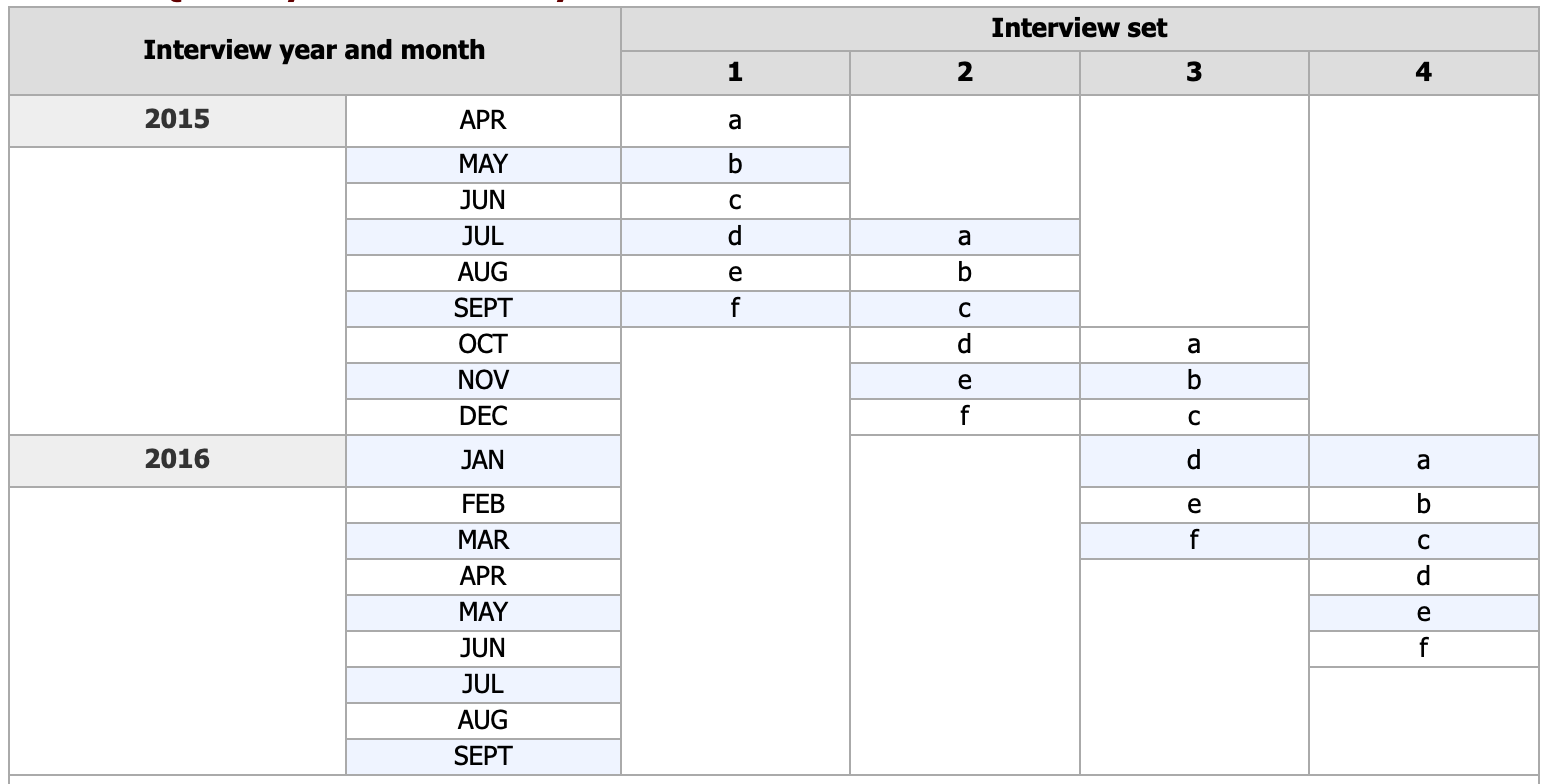
\includegraphics[width=.9\linewidth]{figures/CEX_rotation_table.png}
    \fnote{Columns show number of interview and a letter signals a specific household. Source: \url{https://www.bls.gov/opub/hom/cex/data.htm}}
    \label{fig:cex_rotation}
\end{figure}
%%%%%
\\ It is important to highlight the limitations set by the usage of CEX data. As mentioned, the main objective of the CEX is to assess what goods the average household consumes to create the goods basket for inflation measurements. This focus results in a lack of interest in dense documentation of household characteristics and income-related variables. For example, the lack of asking for liquidity-related measures in each quarter prevents us from controlling for changes in liquidity, but we can only control for households' overall self-reported levels of liquidity and the variables collected are only crude measures for liquidity (Parker et al., 2013). \\
While this is a disadvantage in comparison with other data sources, the CEX's richness in information on consumption behavior is unmatched. Keeping in mind the risk of measurement error through the self-reported consumption measurement, the CEX enables us to analyze not only the MPC for overall consumption but to dissect it and see which goods drive responses and heterogeneity seen in higher level estimates.